%%%%%%%%%%%%%%%%%%%%%%%%%%%%%%%%%%%%%%%%%%%%%%%%%%%%%%%%%%%%%%%%%%%%%%%%%%%%%%%%%%%%%%%%%%%%%%%%%%%%%%%
%%%%%%%%%%%%%% Template de Artigo Adaptado para Trabalho de Diplomação do ICEI %%%%%%%%%%%%%%%%%%%%%%%%
%% codificação UTF-8 - Abntex - Latex -  							     %%
%% Autor:    Fábio Leandro Rodrigues Cordeiro  (fabioleandro@pucminas.br)                            %% 
%% Co-autor: Prof. João Paulo Domingos Silva  e Harison da Silva                                     %%
%% Revisores normas NBR (Padrão PUC Minas): Helenice Rego Cunha e Prof. Theldo Cruz                  %%
%% Versão: 1.0     13 de março 2014                                                                  %%
%%%%%%%%%%%%%%%%%%%%%%%%%%%%%%%%%%%%%%%%%%%%%%%%%%%%%%%%%%%%%%%%%%%%%%%%%%%%%%%%%%%%%%%%%%%%%%%%%%%%%%%
\section{\esp Introdução}

A estimativa da Associação Nacional dos Fabricantes de Veículos Automotores~\cite{ANFAVEA2020} é que no final do ano de 2019 mais de 45 milhões de veículos circularam pelas ruas do Brasil. Em 2018 o setor movimentou mais de 61,9 bilhões de reais e empregou cerca de 1,3 milhões de pessoas diretamente e indiretamente \cite{ANFAVEA2020}. Contudo, de acordo com a Confederação Nacional das Empresas de Seguros Gerais, Previdência Privada e Vida, Saúde Suplementar e Capitalização (CNseg), apenas 30\% frota de veículos brasileira possui algum tipo de proteção veícular \cite{CNseg2019}. Esse número baixo de veículos segurados pode ser explicado devido aos altos custos para manter um veículo no Brasil, como mostra um estudo realizado pela agência Autoinforme, realizada em 2015, onde o valor médio mensal gasto pelo brasileiro com o veículo ultrapassa os 1100 reais \cite{Barros2015}

A maioria das empresas prestadoras de proteção veícular, oference junto aos seus serviços de furto e roubo ou demais sinistros, alguns serviços extras como guincho 24 horas, chaveiro, socorro mecânico entre outros. Outra vantagem oferecida pelas empresas, é a assitência mecânica através de uma rede de oficinas credenciadas por elas. 

Uma pesquisa da revista WebMotors com mais de oito mil pessoas, chegaram a um resultado que mais de 70\% dos entrevistados preferem utilizar oficinas particulares do que os serviços como os das concessionária. Para os entrevistados, o que possui maior peso na hora de escolher uma oficina é o preço mais baixo do serviço e a opção de escolher um mecânico de confiança \cite{Bandeira2019}. Com isso podemos dizer que poucas pessoas possuem acesso à serviços exclusivos das seguradoras além de preferirem procurar serviços em oficinas particulares, devido aos custos dos serviços, preferência por mecânicos de confiança ou outros motivos.

Além da baixa quantidade de pessoas com acessos a esses serviços, o mercado não dispõem aplicativos gratuitos, fora da cobertura de seguradoras, que ofereça essa gama de serviços para usuários que estejam a procura de oficinas mecânicas de qualidade e de serviços de socorro automotivo.

Portanto, este trabalho tem como objetivo, desenvolver um aplicativo móvel que permita usuários buscarem serviços automotivos diversos, desde a solicitação de um guincho ou um socorro de recarga de bateria, até a busca de oficinas especializadas com a possibilidade de realização de orçamento online através de imagens retiradas pelos usuários. Assim permitindo que pessoas que não possuem serviços de seguradoras ou mesmo aquelas que possuem e optem por serviços particulares, possam encontrar serviços especializados de maneira rápida, fácil e que consigam selecionar prestadores que possuem boas reputações no mercado.

Este trabalho será divido nas seguintes seções...



\section{\esp Revisão de literatura}

Tãn nãn nãn...

\subsection{\esp Satisfação de usuários com serviços de seguradoras}



\subsection{\esp }


\subsection{\esp Comparativo entre serviços prestados pelas seguradoras}

Nesta seção, foram selecionados as três maiores segurados, em volume de segurados, para comparar os serviços que eles prestam para os seus clientes. As empresas selecionadas foram o Bradesco Seguros, Tokio Marine e Porto Seguro. Todas as três oferecem cobertura a furto e roubo, danos a terceiros, incêndio e danos ao veículo do segurado, mas a intenção desta pesquisa é destacar os serviços extras oferecidos pelas empresas selecionadas.
\newline

\textbf{Benefícios da seguradora Tokio Marine:}

* Atendimento em todo o território nacional 24 horas por dia.

* Serviço de vidros Básico, Completo ou VIP.

* Contato com o Cliente via telefone, e-mail e SMS, para acompanhamento do sinistro.

* Reboque do veículo segurado (com opções para ampliação da quilometragem).

* Socorro mecânico.

* Meio de transporte alternativo.

* Hospedagem.

* Serviço de Chaveiro.

* Substituição de pneus.

* Entre outros.
\newline

\textbf{Benefícios da seguradora Bradesco Seguros:}

* Assistência Auto Dia e Noite com diversas opções de limites de quilometragens.

* Descontos e serviços gratuitos na DPaschoal, um dos maiores centros automotivos do Brasil.

* Bradesco Auto Center: Tenha acesso a vários serviços automotivos em um único lugar.

* Despachante: Conte com o serviço de despachante no atendimento de sinistro

* Clube de Vantagens Bradesco Seguros

* Descontos em lojas on-line e em estabelecimentos conveniados em todo o país.
\newline

\textbf{Benefícios da seguradora Porto Seguro:}

* Assistência 24 horas: Atendimento a qualquer hora do dia ou da noite, mais guincho sem limite de km.

* Serviços gratuitos para sua casa: Mão de obra para reparos elétricos, hidráulicos, desentupimento, chaveiro 24h e mais.

* Descontos em estacionamentos: Aproveite até 30\% de desconto em mais de 800 estacionamentos em todo país.

* Oficinas com serviços gratuitos: Conte com diagnósticos gratuitos nos Centros Automotivos Porto Seguro.



\section{\esp Trabalhos relacionados}


\section{\esp Metodologia}

O desenvolvimento da aplicação móvel AutoJá, foi dividida em algumas etapas, e a primeira delas foi a concepção das funcionalidades do sistema e a elaboração de um diagrama de casos de uso. Os casos de usos estão ilustrados na Figura 1, e com eles é possível entender o relacionamento das principais funcionalidades do sistema com os seus usuários.

% Figura
\begin{figure}[!ht]
	\centering	
	\caption[\hspace{0.1cm}]{Diagrama de casos de uso do aplicativo AutoJá}
	\vspace{-0.4cm}
	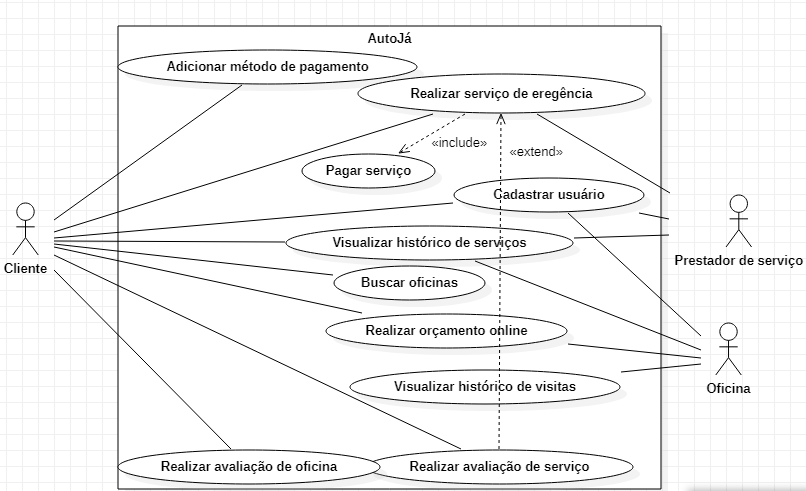
\includegraphics[width=1\textwidth]{figuras/caso_de_uso_autoja.png}
	% Caption centralizada
% 	\captionsetup{justification=centering}
	% Caption e fonte 
	 \vspace{-0.2cm}
	\\\textbf{\footnotesize Fonte: Autor }
	\label{fig:figura1}
\end{figure}
\vspace{-0.5cm}

\subsection{Requisitos do sistema}

A seguir foram listados os requisitos funcionais (Tabela 1) e os requisitos não funcionais (Tabela 2), para nos da uma visão das funcionalidades pretendidas do sistema.

\begin{table}[!ht]
  \begin{center}
    \caption{Requisitos funcionais.}
    \label{tab:table2}
    \begin{tabular}{|c|l|} 
      \hline
      \textbf{ID} & \textbf{Descrição}\\
      \hline
      RF 001 & Cadastro de usuário \\
      \hline
      RF 002 & Autenticação do usuário \\
      \hline
      RF 003 & Atualização de dados cadastrais do usuário \\
      \hline
      RF 004 & Adicionar método de pagamento \\
      \hline
      RF 005 & Buscar serviço de emergência \\
      \hline
      RF 006 & Aceitar serviço de emergência \\
      \hline
      RF 007 & Finalizar serviço de emergência\\
      \hline
      RF 008 & Avaliar profissional \\
      \hline
      RF 009 & Avaliar cliente \\
      \hline
      RF 010 & Visualizar histórico de serviços \\
      \hline
      RF 011 & Buscar oficinas mecânicas \\
      \hline
      RF 012 & Realizar orçamento online \\
      \hline
      RF 013 & Avaliar oficinas mecânicas \\
      \hline
      RF 014 & Favoritar oficinas mecânicas \\
      \hline
      RF 015 & Visualizar histórico de visitas \\
      \hline
      RF 016 & Visualizar avaliações \\
      \hline
      RF 017 & Realizar pagamento \\
      \hline
    \end{tabular}
  \end{center}
\end{table}

\begin{table}[!ht]
  \begin{center}  
    \caption{Requisitos não funcionais.}
    \label{tab:table1}
    \begin{tabular}{|c|l|} 
      \hline
      \textbf{ID} & \textbf{Descrição}\\
      \hline
      RNF 001 & O aplicativo deve ser multiplataforma, funcionando             nos sistemas operacionais \\ 
              & Android e IOS. \\
      \hline
      RNF 002 & O aplicativo deve permitir autenticação pelas contas           do Facebook e do Google. \\
      \hline
      RNF 003 & O tempo máximo de espera para que um prestador de              serviço aceite a solicitação \\
              & não deve exceder 1                minuto em horário    de pico, de 08:00 até 19:00. E não           exceder \\
              & 3 minutos no restante do dia. \\
     \hline
    \end{tabular}
  \end{center}
\end{table}

\subsection{Modelo da arquitetura do sistema}

O próximo passo realizado no desenvolvimento, foi a escolha das tecnologias a serem utilzidas. A primeira delas foi a do \textit{Front-end}, o \textit{framework} Flutter, capaz de executar nativamente nos sistemas operacionais Android e IOS com apenas um código.

Para ilustrar as conexões entre as tecnologias, a figura abaixo (Figura 2), demonstra uma visão geral da solução contendo os principais componentes da arquitetura.

